\renewcommand{\theequation}{\theenumi}
\renewcommand{\thefigure}{\theenumi}
\renewcommand{\thetable}{\theenumi}
\begin{enumerate}[label=\thesection.\arabic*.,ref=\thesection.\theenumi]
\numberwithin{equation}{enumi}
\numberwithin{figure}{enumi}
\numberwithin{table}{enumi}

\item Two players A, and B alternately keep rolling a fair dice. The person to get a six first wins the game. Given that player A starts the game, the probability that A wins the game is:\\[5pt]
\begin{enumerate}[label=(\Alph*)]
    \item $\dfrac{5}{11}$\\
    \item $\dfrac{1}{2}$ \\
    \item $\dfrac{7}{13}$\\
    \item $\dfrac{6}{11}$
\end{enumerate}
\solution
\begin{itemize}
    \item Given the die is fair.
    \item So, for any given throw by A or B:\\
    The probability of getting 6 = $\dfrac{1}{6}$ = p (say)\\
    The probability of NOT getting 6 = $\dfrac{5}{6}$ = q (say)
\end{itemize}
Constraint: A starts the game and A should win.\\
$\implies$ Until A wins, both A and B cannot win.\\
%$\implies$ B(State 2) is absorbing state and it represents the state A loses and B wins.\\
\begin{figure}[!htb]
Corresponding Markov chain is:\\
\begin{center}
    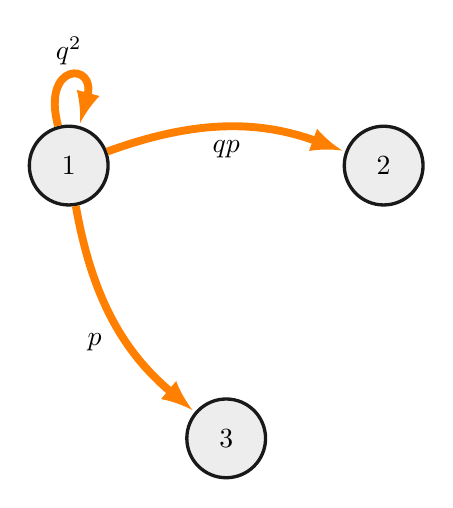
\begin{tikzpicture}[roundnode/.style={circle, draw=black!90, fill=black!7, very thick, minimum size=1cm}]
        \node [roundnode] at (0, 0)     (a)     {1};
        \node [roundnode] at (4, 0)     (b)     {2};
        \node [roundnode] at (2, -3.4641) (w) {3};
        \draw[every loop, auto=right, line width=1mm,
                >=latex, draw=orange,fill=orange]
            (a) edge[bend left=20] node {$qp$} (b)
            (a) edge[loop above=40] node {$q^2$} (a)
            (a) edge[bend right=20] node {$p$} (w);
    \end{tikzpicture}
%        \caption{Modified Markov chain}
        \label{fig:Fig1}
\end{center}
\end{figure}
\begin{table}[!htb]
    \begin{center}
    \begin{tabular}{|c|c|}
        \hline
        State & Corresponding description \\
        \hline
        1 & A and B both lose.\\
        \hline
        2 & A loses and B wins.\\
        \hline
        3 & WINNER\\
        \hline
      \multicolumn{2}{c}{Table 1: State description table}
    \end{tabular}
    \end{center}
\end{table}
\begin{definition}
    \vspace{2cm}
    2 and 3 are ABSORBING states.\\
    Transition/Stochastic matrix is: T\\
    \centering
         \text{\small (From)} \begin{blockarray}{ cccc }
                \multicolumn{3}{c}{(\small To)}\\
                & 1 & 2 & 3 \\
                \begin{block}{ c @{\quad} [ @{\,} *{3}{c} @{\,} ] }
                    1 & $q^2$ & qp & p\\ 
                    2 & 0 & 1 & 0\\
                    3 & 0 & 0 & 1\\
                \end{block}
           \end{blockarray} = T
\end{definition}
\begin{theorem}
Every transition matrix can be partitioned as $\mleft(
    \begin{array}{c|c}
        Q & P\\
        \hline
        O & J\\
    \end{array}
    \mright)$\\
    where Q arise from transition probabilities between non-absorbing states\\
    R arises from Transition probability from non-absorbing state to absorbing state.\\
    O = Null matrix,
    J = Identity matrix\\
    $T^k$ approaches $\overline{T}$ as k increases.
    $\overline{T}$ is the limiting matrix and
    $\overline{T} = \myvec{O & NP\\O & J}$\\
    where N is the fundamental matrix.
    $N = (I - Q)^{-1}$\\
    \end{theorem}
\begin{definition}
    The matrix D = NP gives the probability of ending up in the absorbing states (2 and 3) when the chain starts from a non-absorbent state 1.
\end{definition}
    \[T = \mleft(
    \begin{array}{c| c c}
        q^2 & qp & p\\
        \hline
        0 & 1 & 0\\
        0 & 0 & 1\\
    \end{array}
    \mright)\]
    \begin{align}
        Q = \myvec{q^2},
        P = \myvec{qp & p},
        O = \myvec{0 \\ 0},
        J = \myvec{1 & 0\\0 & 1} \label{eq:eqn1}
    \end{align}

    \begin{align}
        N = \myvec{1 - q^2}^{-1} = \myvec{\dfrac{1}{1-q^2}}\\
        D = NP = \myvec{\dfrac{qp}{1 - q^2} & \dfrac{p}{1 - q^2}}\\
        \pr{\text{A wins}} = D_2 = \dfrac{p}{1 - q^2} = \frac{\frac{1}{6}}{1 - \frac{25}{36}} = \dfrac{6}{11}
    \end{align}
        \centering
\[
    \pr{\text{A wins}} = \dfrac{6}{11}
\]
OPTION D is correct


\item A fair coin is tossed till a head appears for the first time. The probability that the number of requried tosses is odd,is
\begin{enumerate}
\begin{multicols}{4}
\setlength\itemsep{2em}
\item $
\dfrac{1}{3}
$
\item $
\dfrac{1}{2}
$
\item $
\dfrac{2}{3}
$
\item $
\dfrac{3}{4}
$
\end{multicols}
\end{enumerate}
\solution
We can see that if the first toss is guaranteed to be a head, then the problem is reduced to finding the probability of getting one head in 2 coin tosses, since all the 3 trials are independent.
Let $K=\{0, 1, 2\}$ be the random variable denoting the number of heads obtained in 2 tosses of a fair coin. The event can be represented by a binomial distribution b(n,p).
In binomial distribution b(n,p), 
\begin{align}
Pr\brak{K=i}= \binom{n}{i}p^i \cdot (1-p)^{n-i}.
\end{align}
Here $n=2, p=0.5$.
 We can see that the probability of $K=1$ is 
 \begin{align}
 Pr\brak{K=1}&=\binom{2}{1} \cdot 0.5^2\\
 &=\frac{1}{2}
 \end{align}
 
From $\brak{2.0.1}$ and $\brak{2.0.2}$, we see that probability of getting exactly 2 heads in 3 tosses, if the first toss is a head, is 0.5.

%
\item A fair coin is tossed till a head appears for the first time. The probability that the number of requried tosses is odd,is
\begin{enumerate}
\begin{multicols}{4}
\setlength\itemsep{2em}
\item $
\dfrac{1}{3}
$
\item $
\dfrac{1}{2}
$
\item $
\dfrac{2}{3}
$
\item $
\dfrac{3}{4}
$
\end{multicols}
\end{enumerate}
%
\solution
Given, a fair coin is tossed till heads turns up.
\begin{align}
\tag{47.1}
\label{markov/1/eq:0}
    p=\dfrac{1}{2},q=\dfrac{1}{2}
\end{align}
    Let us define a Markov chain $\{X_{0},X_{1},X_{2}\dots\}$, where $X_{n}\in S=\{1,2,3,4\}$ where $n\in \{0,1,2,\dots\}$, 
\begin{table}[h!]
\centering
\caption{Definition of Random Variables}
\label{markov/1/table:1}
\begin{tabular}{|c|c|c|}
    \hline
    R.V & Value=0 & Value=1 \\
    \hline
    $X$ & $N_{tosses}=2k$ & $N_{tosses}=2k-1$ \\[1ex]
    \hline
    $Y$ & $H$ & $T$ \\[1ex]
    \hline
\end{tabular}
\end{table}    
\begin{table}[h!]
\centering
\caption{Markov states and Notations }
\label{markov/1/table:2}
\begin{tabular}{|c|c|}
    \hline
    Notation & State \\
    \hline
    $S=1$ & $(X,Y)=(0,1)$ \\[1ex]
    \hline
    $S=2$ & $(X,Y)=(1,1)$\\[1ex]
    \hline
    $S=3$ & $(X,Y)=(0,0)$\\[1ex]
    \hline
    $S=4$ & $(X,Y)=(1,0)$\\[1ex]
    \hline
\end{tabular}
\end{table}
\begin{figure}[h]
\caption*{\textbf{Markov chain diagram}}
\centering
\begin{tikzpicture}
    % Setup the style for the states
        \tikzset{node style/.style={state, 
                                    minimum width=1.5cm,
                                    line width=1mm,
                                    fill=gray!20!white}}
        % Draw the states
        \node[node style] at (3, -4)      (bull) {1};     
        \node[node style] at (0, -8)      (bear) {2};      
        \node[node style] at (6, -8)     (over1) {3};  
        \node[node style] at (3, 0)      (over2) {4}; 
        % Connect the states with arrows
        \draw[every loop,
              auto=right,
              line width=0.7mm,
              >=latex,
              draw=orange,
              fill=orange]
        (bull) edge[bend right = 20] node{$\frac{1}{2}$} (bear)
        (bear) edge[bend right = 20] node{$\frac{1}{2}$}
        (bull)
        (bear) edge[bend right = 20] node{$\frac{1}{2}$}
        (over1)
        (over1) edge[loop below] node{1}
        (over1)
        (bull) edge node{$\frac{1}{2}$} (over2)
        (over2) edge[loop above] node{1} (over2) ;
\end{tikzpicture}
\end{figure}
\newpage
\begin{definition}
The standard form of a state transition matrix is,
\begin{align}
\tag{47.2}
\label{markov/1/eq:std}
   \vec{P}=\begin{blockarray}{ccc}
&A & N \\
\begin{block}{c[cc]}
  A & \vec{I} & \vec{O}  \\
  N & \vec{R} & \vec{Q} \\
\end{block}
\end{blockarray}
\end{align}
where,
\begin{table}[h!]
\centering
\caption{Notations and their meanings}
\label{markov/1/table:3}
\begin{tabular}{|c|c|}
    \hline
    Notation & Meaning \\
    \hline
    $A$ & Absorbing states (3,4)\\[1ex]
    \hline
    $N$ & Non-absorbing states (1,2)\\[1ex]
    \hline
    $\vec{I}$ & Identity matrix\\[1ex]
    \hline
    $\vec{O}$ & Zero matrix\\[1ex]
    \hline
    $\vec{R},\vec{Q}$ & Other sub-matrices\\[1ex]
    \hline
\end{tabular}
\end{table}
\end{definition}
\begin{corollary}
The state transition matrix for the above Markov chain is, 
\begin{align}
\tag{47.3}
\label{markov/1/eq:pstd}
    \vec{P}=\begin{blockarray}{cccccc}
& 3 & 4 & 1 & 2 \\
\begin{block}{c[ccccc]}
  3 & 1 & 0 & 0 & 0 \\
  4 & 0 & 1 & 0 & 0 \\
  1 & 0 & 0.5 & 0 & 0.5  \\
  2 & 0.5 & 0 & 0.5 & 0  \\
\end{block}
\end{blockarray}
\end{align}
\end{corollary}
From \eqref{markov/1/eq:pstd},
\begin{align}
\tag{47.4}
\label{markov/1/eq:r,q}
    \vec{R}=\begin{bmatrix}
    0 & 0.5\\
    0.5 & 0\\
    \end{bmatrix},
    \vec{Q}=\begin{bmatrix}
    0 & 0.5 \\
    0.5 & 0 \\
    \end{bmatrix}
\end{align}
\begin{definition}
The limiting matrix for absorbing Markov chain is,
\begin{align}
\tag{47.5}
\label{markov/1/eq:pbar}
    \vec{\bar P}=\begin{bmatrix}
    \vec{I} & \vec{O}\\
    \vec{FR} & \vec{O}\\
    \end{bmatrix}
\end{align}
\\where,
\begin{align}
\tag{47.6}
\label{markov/1/eq:f}
    \vec{F}=(\vec{I}-\vec{Q})^{-1}
\end{align}
is called the fundamental matrix of $\vec{P}$. \\
\end{definition}
\begin{corollary}
Limiting Matrix of the Markov chain under observation is, 
\begin{align} 
\tag{47.7}
\label{markov/1/eq:ans}
    \vec{\bar P}=\begin{blockarray}{ccccc}
&3 &4 &1 &2\\
\begin{block}{c[cccc]}
    3 & 1 & 0 & 0 & 0  \\
    4 & 0 & 1 & 0 & 0  \\
    1 & \frac{1}{3} & \frac{2}{3} & 0 & 0 \\
    2 & \frac{2}{3} & \frac{1}{3} & 0 & 0 \\
   \end{block}
\end{blockarray}
\end{align}
\end{corollary}
\begin{definition}
A element $\bar p_{ij}$ of $\vec{\bar P}$ denotes the absorption probability in state $j$, starting from state $i$.
\end{definition}
\begin{corollary}
The required probability is,
\begin{align}
\tag{47.8}
\label{markov/1/eq:ams}
P =\bar p_{14}
\end{align}
From \eqref{markov/1/eq:ans} and \eqref{markov/1/eq:ams},
\begin{align}
\tag{47.9}
P=\frac{2}{3}
\end{align}
\end{corollary}
Therefore, option 3 is correct.

%



\item \textbf{Step 1.} Flip a coin twice.\\
\textbf{Step 2.} If the outcomes are (TAILS, HEADS) then output Y and stop.\\
\textbf{Step 3.} If the outcomes are either (HEADS, HEADS) or (HEADS, TAILS), then output N and stop.\\
\textbf{Step 4.} If the outcomes are (TAILS, TAILS), then go to Step 1.\\
The probability that the output of the experiment is Y is (upto two decimal places)......
\\
%
\solution
Let flipping a coin twice be event H.\\
Sample space of event H = \cbrak{HH,HT,TH,TT}\\
Let a random variable X; $X_{i}=i$, where i=1,2,3. \\
 $X_{1}$ represents outcome \cbrak{TT}, 
 \\$X_{2}$ represents getting outcome \cbrak{TH} or output Y,
 \\ $X_{3}$ represents getting output N.\\
The state transition matrix P is shown below :
\begin{align}
\begin{array}{c c} &
\begin{array}{c c c} X_{1}  & X_{2} & X_{3} \\
\end{array}
\\
\begin{array}{c c c}
X_{1} \\
X_{2}\\
X_{3}
\end{array}
&
\left[
\begin{array}{c c c}
\frac{1}{4} & \frac{1}{4} & \frac{1}{2} \\
0 & 1 & 0 \\
0 & 0 & 1 
\end{array}
\right]
\end{array}
\end{align}
\\
\begin{figure}[h]
\caption*{\textbf{Markov chain diagram}}
\centering
\begin{tikzpicture}
       
             % Setup the style for the states
        \tikzset{node style/.style={state, 
                                    minimum width=1cm,
                                    line width=0.7mm,
                                    fill=gray!20!white}}
        % Draw the states
        \node[node style] at (3, 0)      (bull)     {$X_{1}$};
        \node[node style] at (0, -3)      (bear)     {$X_{2}$};
        \node[node style] at (6, -3) (stagnant) {$X_{3}$};
        % Connect the states with arrows
        \draw[every loop,
              auto=right,
              line width=0.7mm,
              >=latex,
              draw=orange,
              fill=orange]
           (bull)     edge[bend left=20]            node {$\frac{1}{2}$} (stagnant)
            (bull)     edge[bend right=20] node {$\frac{1}{4}$} (bear)
            
            
            (bull) edge[loop above]             node  {$\frac{1}{4}$} (bull)
            (bear) edge[loop below]             node  {1} (bear)
            (stagnant) edge[loop below]             node  {1} (stagnant);
    \end{tikzpicture}
\end{figure}\\
From the transition matrix, we have 1 transient state and 2 absorbing states.\\ Q = $\begin{bmatrix} \frac{1}{4} \end{bmatrix}$ and R = $\begin{bmatrix} \frac{1}{4} & \frac{1}{2} \end{bmatrix}$
\begin{align}
 N ={}& \brak{I - Q}^{-1}\\
 ={}& \brak{\sbrak{1} - \sbrak{\frac{1}{4}}}^{-1}\\
 ={}& \sbrak{\frac{4}{3}}
\end{align}
We know that probability of being absorbed by state j after starting in state i is given by the $M_{i,j}$, where M = NR.\\
\begin{align}
M = \begin{bmatrix} \frac{1}{3} & \frac{2}{3} \end{bmatrix}
\end{align}.\\
 Hence the probability of being absorbed by state Y $\brak{1^{st} \text{element of R}}$ after starting with state $X_{1}\brak{1^{st}\text{element of Q}}$ is $M_{1,1}$\\
 \\
\begin{align}
\therefore \pr{Y}=\frac{1}{3}=0.33 \brak{\text{correct upto 2 decimal places}}.
\end{align}


%
\item Players A and B take turns to throw a fair dice with six faces. If A is the first player to throw, then the probability of B being the first one to get a six is --- ( round of to two decimal places). \\
\solution

Let the random variable X represent which player gets six first. That is $X=0 $ when A gets a six first and $X=1 $ when B gets six first. \\
Let another random variable Y represent getting a six on the dice. $Y=1 $ for six and $Y=0 $ for any other number. \\
Let N be the number of turns until we get a six.
\begin{align}
    \Pr\brak{Y=0} = \frac{5}{6} \\
    \Pr\brak{Y=1} = \frac{1}{6}
\end{align}
The event success is when B gets a six for first time and failure is when neither A nor B gets six. Let p denote probability of success 
\begin{align}
    p &= \Pr\brak{Y=1}  \\
    \Pr\brak{Y=0} &= 1- p \\
    p &= \frac{1}{6}
\end{align}
To get $X=1 $ in $N$ turns we have to get $N-1$ failures for B and $ N$ failures for A and finally one success for B. 
Therefore the geometric distribution is,
\begin{align}
    f(N) &= \brak{1-p}^{n-1} \times p \times  \brak{1-p}^{n} \\
    &  = \brak{1-p}^{2n-1} \times p \\
    & = \brak{ \frac{5}{6}}^{2n-1} \times \frac{1}{6}
\end{align}
The result has been summarized in table \ref{tab:table geometric distribution}. \\
\begin{table}[hbt!]
\centering
\begin{tabular}{|c|c|}
\hline
\textbf{No. of turns} & \textbf{Probability} \\ \hline
1                     & $5^1/6^2  $            \\ \hline
2                     & $5^3/6^4 $             \\ \hline
$\vdots  $              & $\vdots $              \\
n                     & $5^{2n-1}/6^{2n} $         \\ \hline
$\vdots $               & $\vdots $              \\ \hline
\end{tabular}
\caption{Summary of turns}
\label{tab:table geometric distribution}
\end{table}
Thus the total probability is sum of these individual probabilities i.e.
\begin{align}
    \Pr\brak{X=1} &= \sum_{N=1}^{\infty} f(N) \\
    &= \frac{5}{6^2} + \frac{5^3}{6^4} + \hdots + \frac{5^{2n-1}}{6^{2n}} +\hdots  \\
    &= \frac{5}{6^2} \times \brak{1 + \frac{5^2}{6^2} + \frac{5^4}{6^4} + \hdots } 
\end{align}
By Using sum of infinite GP we have, 
\begin{align}
     \Pr\brak{X=1} &= \frac{5}{6^2} \times \brak{\frac{1}{1 - \frac{25}{36}}}  \\
       &= \frac{5}{36} \times \frac{36}{11} \\
       &= \frac{5}{11} = 0.45
\end{align}
%
\item A fair coin is tossed till a head appears for the first time. The probability that the number of requried tosses is odd,is\\
\begin{enumerate}
    \item $\dfrac{1}{3}$\\
    \item $\dfrac{1}{2}$\\
    \item $\dfrac{2}{3}$\\
    \item $\dfrac{3}{4}$
\end{enumerate}
\solution
  
A sequence of random variables $Y_1,Y_2,Y_3\hdots$ converges, in probability, to a random variable $Y$ if
\begin{align}
    \lim_{n\rightarrow \infty}\Pr{(\abs{Y_n-Y}\geq \epsilon)} = 0 \quad \forall \epsilon >0
\end{align}
Similarly, a sequence of random variables $Y_1,Y_2,Y_3\hdots$ converges, in mean square, to a random variable $Y$ if
\begin{align}
    \lim_{n\rightarrow \infty} E(\abs{Y_n-Y}^2) = 0 
\end{align}
A random variable converges, in probability, to a value if it converges, in mean square, to the same particular value by Markov's Inequality. Proof for this is: For any $\epsilon > 0$
\begin{align}
    \Pr{(\abs{Y_n-Y}\geq \epsilon)} = \Pr{(\abs{Y_n-Y}^2\geq \epsilon^2)}
\end{align}
\begin{multline}
    \Pr{(\abs{Y_n-Y}\geq \epsilon)}  \leq \frac{E\abs{Y_n-Y}^2}{\epsilon^2} 
    \\\text{ (by Markov's Inequality)}
\end{multline}
 
\begin{align}
    \lim_{n\rightarrow \infty} E(\abs{Y_n-Y}^2) = 0 
    \\0 \leq  \lim_{n\rightarrow \infty}\Pr{(\abs{Y_n-Y}\geq \epsilon)}  \leq \frac{0}{\epsilon^2}
    \\   \lim_{n\rightarrow \infty}\Pr{(\abs{Y_n-Y}\geq \epsilon)} = 0 \quad \forall \epsilon >0
\end{align}
Given in the question that $\{X_j\}$ is a sequence of random variables with
\begin{align}
    \Pr{(X_j=1)} = \frac{1}{4}
    \\\Pr{(X_j=0)} + \Pr{(X_j=1)} = 1
    \\\Pr{(X_j=0)} = 1 - \frac{1}{4} = \frac{3}{4}
\end{align}
\begin{align}
    X_j \in \{0,1\} 
\end{align}
Since $0^2 = 0$ and $1^2 = 1$, 
\begin{align}
    X_j^2 = X_j \quad \forall j \in \{1, 2,\hdots, n\}
\end{align}
Thus, 
\begin{align}
    Y_n &= \frac{1}{n} \sum_{j=1}^{n}X_j^2 
    \\&= \frac{1}{n} \sum_{j=1}^{n}X_j
    \\\Pr{(Y_n = y)} &= \comb{n}{ny} \brak{\frac{1}{4}}^{ny} \brak{\frac{3}{4}}^{n-ny}
\end{align}
Let us assume
\begin{align}
    k &= ny
    \\k &\in \{0,1,2,\hdots,n-1,n\}
    \\ \Pr{(Y_n = \frac{k}{n})} &= \comb{n}{k} \brak{\frac{1}{4}}^{k} \brak{\frac{3}{4}}^{n-k}
\end{align}
\begin{align}
    E\brak{\abs{Y_n-\frac{1}{4}}^2} &= E\brak{Y_n^2 - \frac{1}{2}Y_n + \frac{1}{16}}
    \\&= E(Y_n^2) - \frac{1}{2}E(Y_n) + \frac{1}{16} \label{ma2018-25:equation 0}
\end{align}
\begin{align}
    E(Y_n^2) &= \sum_{k=0}^n\brak{\frac{k}{n}}^2\Pr{\brak{Y_n=\frac{k}{n}}}
    \\&= \sum_{k=0}^{n} \brak{\frac{k^2}{n^2}}\comb{n}{k} \brak{\frac{1}{4}}^{k} \brak{\frac{3}{4}}^{n-k}
\end{align}
\begin{multline}
    E(Y_n^2) = 0 + \frac{1}{n^2}\times n\brak{\frac{1}{4}}^{1} \brak{\frac{3}{4}}^{n-1} + \\\sum_{k=2}^{n} \brak{\frac{k}{n}}^2\times\frac{n(n-1)}{k(k-1)}
    \times\comb{n-2}{k-2}\brak{\frac{1}{4}}^{k} \brak{\frac{3}{4}}^{n-k}
\end{multline}
\begin{multline}
    E(Y_n^2) =  \frac{1}{4n}\brak{\frac{3}{4}}^{n-1} + \frac{n-1}{n} 
   \\\times\sum_{k=2}^{n} \brak{\frac{k}{k-1}}\comb{n-2}{k-2}\brak{\frac{1}{4}}^{k} \brak{\frac{3}{4}}^{n-k}
\end{multline}
\begin{multline}
    E(Y_n^2)  = \frac{1}{4n}\brak{\frac{3}{4}}^{n-1} \\+ \frac{n-1}{n} 
   \brak{\sum_{k=2}^{n}\comb{n-2}{k-2}\brak{\frac{1}{4}}^{k} \brak{\frac{3}{4}}^{n-k} }
   \\+\frac{n-1}{n} \brak{\sum_{k=2}^{n}\frac{1}{k-1}\comb{n-2}{k-2}\brak{\frac{1}{4}}^{k} \brak{\frac{3}{4}}^{n-k} } 
\end{multline}
\begin{multline}
    E(Y_n^2)  = \frac{1}{4n}\brak{\frac{3}{4}}^{n-1} + \frac{n-1}{n}\\ \times\frac{1}{16} 
   \brak{\sum_{k=2}^{n}\comb{n-2}{k-2}\brak{\frac{1}{4}}^{k-2} \brak{\frac{3}{4}}^{(n-2)-(k-2)} }
   \\+\frac{1}{n} \brak{\sum_{k=2}^{n}\frac{n-1}{k-1}\comb{n-2}{k-2}\brak{\frac{1}{4}}^{k} \brak{\frac{3}{4}}^{n-k} }
\end{multline}
\begin{multline}
     E(Y_n^2)= \frac{1}{4n}\brak{\frac{3}{4}}^{n-1} \\+ \frac{n-1}{16n} 
   \brak{\sum_{j=0}^{n-2}\comb{n-2}{j}\brak{\frac{1}{4}}^{j} \brak{\frac{3}{4}}^{(n-2)-j} }
   \\+\frac{1}{4n} \brak{\sum_{k=2}^{n}\comb{n-1}{k-1}\brak{\frac{1}{4}}^{k-1} \brak{\frac{3}{4}}^{(n-1)-(k-1)} } 
\end{multline}
\begin{multline}
    E(Y_n^2) = \frac{1}{4n}\brak{\frac{3}{4}}^{n-1} + \frac{n-1}{16n}\brak{\frac{1}{4} + \frac{3}{4}}^{n-2}
   \\+\frac{1}{4n} \brak{\sum_{j=1}^{n-1}\comb{n-1}{j}\brak{\frac{1}{4}}^{j} \brak{\frac{3}{4}}^{(n-1)-j} }
\end{multline}
\begin{multline}
   E(Y_n^2) = \frac{1}{4n}\brak{\frac{3}{4}}^{n-1} + \frac{n-1}{16n}
   \\+\frac{1}{4n} \brak{\brak{\frac{1}{4} + \frac{3}{4}}^{n-1} - \brak{\frac{3}{4}}^{n-1}} 
\end{multline}
\begin{align}
    E(Y_n^2) &= \frac{1}{4n}\brak{\frac{3}{4}}^{n-1} + \frac{n-1}{16n} +\frac{1}{4n} - \frac{1}{4n}\brak{\frac{3}{4}}^{n-1}
    \\&= \frac{1}{16} + \frac{3}{16n} \label{ma2018-25:equation 2}
\end{align}
\begin{align}
    E(Y_n) &= \sum_{k=0}^n\frac{k}{n}\Pr{\brak{Y_n=\frac{k}{n}}}
    \\&= \sum_{k=0}^{n} \brak{\frac{k}{n}}\comb{n}{k} \brak{\frac{1}{4}}^{k} \brak{\frac{3}{4}}^{n-k}
    \\&= 0 + \sum_{k=1}^{n} \frac{k}{n}\times\frac{n}{k}\times\comb{n-1}{k-1}\brak{\frac{1}{4}}^{k} \brak{\frac{3}{4}}^{n-k}
    \\&= \frac{1}{4}\sum_{j=0}^{n-1} \comb{n-1}{j}\brak{\frac{1}{4}}^{j} \brak{\frac{3}{4}}^{(n-1)-j}
    \\&= \frac{1}{4}\brak{\frac{1}{4} + \frac{3}{4}}^{n-1}
    \\&= \frac{1}{4} \label{ma2018-25:equation 3}
\end{align}
Using equations \eqref{ma2018-25:equation 2} and \eqref{ma2018-25:equation 3} in \eqref{ma2018-25:equation 0},
\begin{align}
    E\brak{\abs{Y_n-\frac{1}{4}}^2} &= \frac{1}{16}+ \frac{3}{16n}-\frac{1}{2}\times\frac{1}{4} + \frac{1}{16}
    \\&= \frac{3}{16n}
\end{align}
\begin{align}
    \lim_{n\rightarrow \infty} E\brak{\abs{Y_n-\frac{1}{4}}^2} &=  \lim_{n\rightarrow \infty}  \frac{3}{16n}
    \\&= \frac{3}{16}\lim_{n\rightarrow \infty}\frac{1}{n}
    \\&= 0
\end{align}
Thus, $Y_n$ converges, in mean square, to $\frac{1}{4}$ and hence $Y_n$ converges, in probability, to $\frac{1}{4}$.
%
\item  Consider the experiment with the following steps.
\begin{enumerate}
\item  Flip a coin twice.
\item If the outcomes are (TAILS, HEADS) then output Y and stop.
\item If the outcomes are either (HEADS, HEADS) or (HEADS, TAILS), then output N and stop.
\item If the outcomes are (TAILS, TAILS), then go to Step 1.
\end{enumerate}
The probability that the output of the experiment is Y is (upto two decimal places)......
\\
\solution 
  Given a fair coin is flipped twice.\\
Let us define a Markov chain with states \{1,2,3,4\}, such that 
\begin{table}[h!]
\resizebox{\columnwidth}{!}{
\begin{tabular}{|c|l|}
\hline
\textbf{State} & \multicolumn{1}{c|}{\textbf{Events}}                     \\ \hline
1                 & Event of tossing a fair coin twice                           \\ \hline
2                 & Event of obtaining 'N' as the output                         \\ \hline
3                 & Event of obtaining 'Y' as the output                         \\ \hline
4                 & Event of obtaining (TAIL,TAIL) as the output                 \\ \hline
\end{tabular}
}
\caption{Representation of different events}
\label{cs/2016/29table:1}
\end{table}
\\We know that when a fair coin is tossed,
\begin{align}
    \pr{\text{HEAD}} &=  1/2 \text{ and }\\
    \pr{\text{TAIL}} &=  1/2.
\end{align}
Then, \\
\begin{figure}
    \centering
    \caption{\textbf{Markov chain diagram}}
    \label{cs/2016/29fig:1}
    \begin{tikzpicture}[font=\sffamily]
        % Setup the style for the states
        \tikzset{node style/.style={state, 
                                    minimum width=2cm,
                                    line width=0.5mm,
                                    fill=gray!20!white}}
        % Draw the states
        \node[node style] at (0, 0)     (2)     {2};
        \node[node style] at (3, 0)     (3)     {3};
        \node[node style] at (6, 0)     (4)     {4};
        \node[node style] at (3, -5)    (1)     {1};
        
        % Connect the states with arrows
        \draw[every loop,
              auto=right,
              line width=1mm,
              >=latex,
              draw=orange,
              fill=orange]
            (1)     edge[bend left=10, auto=left]  node {0.5} (2)
            (1)     edge                node {0.25} (3)
            (1)     edge[bend right=10, auto=right] node {0.25} (4)
            (4)     edge[bend left=50, auto=left]            node {1} (1)
            (3)     edge[loop above]                node {1} (3)
            (2)     edge[loop above]                node {1} (2)
            ;
\end{tikzpicture}
\end{figure}
The state transition matrix (P) for the Markov chain is
\begin{align}
\label{cs/2016/29eq:1}
    P=\begin{blockarray}{ccccc}
& 1 & 2 & 3 & 4 \\
\begin{block}{c[cccc]}
  1 & 0 & \frac{1}{2} & \frac{1}{4}  & \frac{1}{4}  \\
  2 & 0 & 1 & 0 & 0 \\
  3 & 0 & 0 & 1 & 0 \\
  4 & 1 & 0 & 0 & 0 \\
\end{block}
\end{blockarray}
\end{align}
By the definition of transient and absorbing states, we can say that 1,4 are transient states whereas 2,3 are absorbing.\\
Then, the canonical form of the transition matrix is,
\begin{align}
\label{cs/2016/29eq:2}
    P=\begin{blockarray}{ccccc}
& 2 & 3 & 1 & 4 \\
\begin{block}{c[cc|cc]}
  2 & 1 & 0 & 0 & 0  \\
  3 & 0 & 1 & 0 & 0 \\ 
  \cline{2-5}
  1 & \frac{1}{2} & \frac{1}{4} & 0 & \frac{1}{4} \\
  4 & 0 & 0 & 1 & 0 \\
\end{block}
\end{blockarray}
\end{align}
The canonical form divides the transition matrix into four sub-matrices based on the states as listed below.\\
\begin{blockarray}{ccc}
& \text{Absorbing} & \text{Non-Absorbing} \\
\begin{block}{c[c|c]}
  \text{Absorbing} & I & O \\
  \cline{2-3}
  \text{Non-Absorbing} & A & B \\
  \end{block}
\end{blockarray}
\\where,
\begin{table}[h!]
\centering
\begin{tabular}{|c|c|}
    \hline
    \textbf{Variable} & \textbf{Type of Matrix} \\
    \hline
    $I$ & Identity matrix\\
    \hline
    $O$ & Zero matrix\\
    \hline
    $A,B$ & Some matrices\\
    \hline
\end{tabular}
\caption{Representation of different matrices}
\label{cs/2016/29table:2}
\end{table}
\\and From \eqref{cs/2016/29eq:2},
\begin{align}
\label{cs/2016/29eq:3}
    A=\begin{bmatrix}
    \frac{1}{2} & \frac{1}{4}\\
    0 & 0\\
    \end{bmatrix},
    B=\begin{bmatrix}
    0 & \frac{1}{4} \\
    1 & 0 \\
    \end{bmatrix}
\end{align}
The fundamental matrix F for the absorbing Markov chain is defined as 
\begin{align}
    F &=(I-B)^{-1} \label{cs/2016/29eq:4}\\
\shortintertext{Then,  }
    F &= \begin{bmatrix}
    1 & -\frac{1}{4} \\
    -1 & 1 \\ 
    \end{bmatrix}^{-1} \\
    \implies F &= \begin{bmatrix}
               1.33 & 0.33 \\
               1.33 & 1.33 \\ 
               \end{bmatrix}\\
\shortintertext{Therefore,}
    FA &= \begin{bmatrix}
    0.67 & 0.33 \\
    0.67 & 0.33 \\ 
    \end{bmatrix}
    \end{align}
Then the limiting matrix for the markov chain is 
\begin{align}
\label{cs/2016/29eq:5}
    \bar P&=\begin{bmatrix}
    I & O\\
    FA & O\\
    \end{bmatrix}
\end{align}
where the element $p_{ij}$ of $\bar P$ represents the probability of absorption in state j, when the initial state is i.
\begin{align}
  \therefore \bar P&=\begin{blockarray}{ccccc}
                  & 2 & 3 & 1 & 4 \\
                  \begin{block}{c[cccc]}
                  2 & 1 & 0 & 0 & 0  \\
                  3 & 0 & 1 & 0 & 0 \\ 
                  1 & 0.67 & 0.33 & 0 & 0 \\
                  4 & 0.67 & 0.33 & 0 & 0 \\
                \end{block}
                \end{blockarray}  
\end{align}
Therefore,
\begin{align}
    \text{ Req. Probability }= p_{13} = 0.33
\end{align}
  Consider a simple symmetric random walk on integers, where from every state i you move to i-1 and i+1 with the probability half each. Then which of the following are true?
  \begin{enumerate}
  \item The random walk is aperiodic
  \item The random walk is irreducible
  \item The random walk is null recurrent 
  \item The random walk is positive recurrent
  \end{enumerate}

\end{enumerate}